\section{Tentative Lines of Research}

\subsection{Networks, Boundaries \& Peformance}

\textbf{\underline {Short Project Description:}} Because of cultural, historical or natural reasons, Countries have the tendency to subdivide its territory in different administrative levels. On the other hand, the functional city-regions are difficult (if not impossible) to define. Transport, Education, Health and so forth cannot be bounded to territory as socio-economic activities happen in different locations. Regional, Provincial, Municipal jurisdictions are fictional boundaries created without taking into consideration urban functions.  \par
This line of research will explore the consequences of spatial compartmentalization. By studying and understanding the spatial relations behind the waste MGMT system there is an opportunity to identify opportunities and threats of the system. \par

\textbf{\underline {Hypothesis:}}  Spatial administrative boundaries are fictional impositions that affect performance negatively.  \par

\textbf{\underline {Exploratory Research Questions: }} 
\begin{itemize}
    \item Should each municipality provide all the services related to waste MGMT or there is place for synergies? 
    \item Under what circumstances the system might under perform and under which ones it will outperform?
    \item Is the service being provided equally across the territory or in border areas there is lower coverage due to shared responsibilities. 
\end{itemize}


\begin{figure}[hbt!]
    \centering
    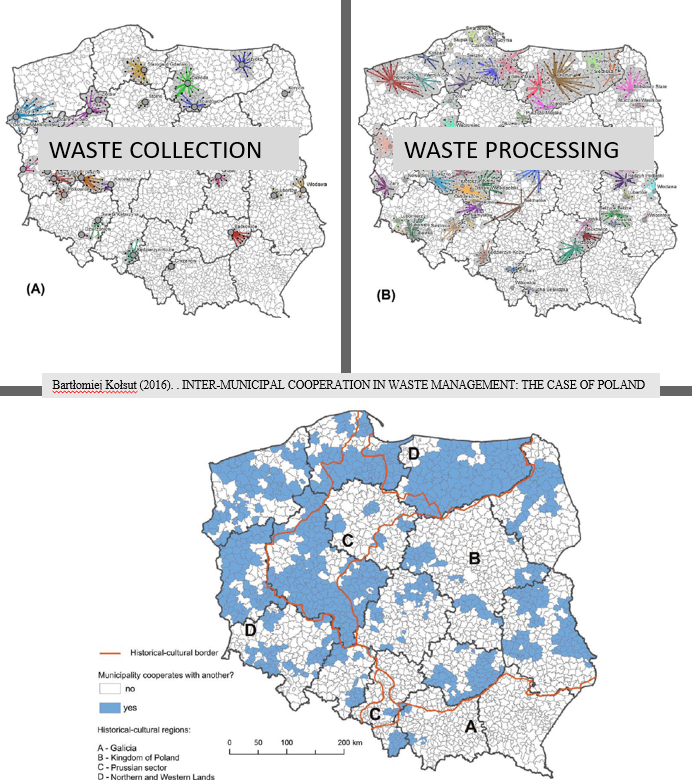
\includegraphics[width=0.5\textwidth]{Imgs/rl_1.PNG}
    \caption{Research Lines 1}
    \label{fig:rl1}
\end{figure}






\subsection{Urban Form, Land Use (Function) and Performance}
\textbf{\underline {Short Project Description:}}  As any other systems, Waste MGMT and food production/distribution have their own set of KPIs to monitor the performance of the systems, fuel costs, time or emissions can be used to understand how well those systems are working. Yet, all these processes are happening somewhere in the City-Region and consequently mapping them and identifying how intensely they relate one to the other is important to improve some of the processes carried out by these systems.
Land Use and how socio-economic activities are distributed across space, might have impact on the performance of these systems. The interrelationships between food generation, food disposal, food consumption, waste generation, waste treatment, waste collection and land use have not been explored as in depth as other systems; for instance, transport and land use.  \par


\textbf{\underline {Hypothesis:}}  Urban and Regional Planning have not fully explored how the spatial distribution of socio-economic activities affect waste MGMT and food systems performance. By spatializing these activities, they would be more easily considerate in planning processes. \par


\textbf{\underline {Exploratory Research Questions: }} 
\begin{itemize}
    \item 	Does each strategy perform differently under different urban form and land use scenarios?
    \item 	Which strategies are better given a specific urban form and function?
\end{itemize}


\begin{figure}[hbt!]
    \centering
    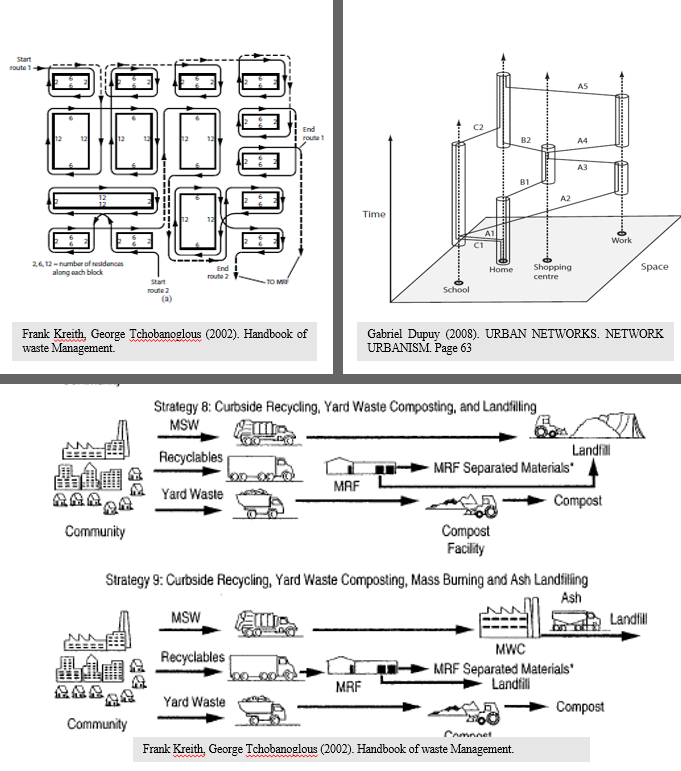
\includegraphics[width=0.5\textwidth]{Imgs/rl_2.PNG}
    \caption{Research Lines 2}
    \label{fig:rl2}
\end{figure}






\subsection{Network characteristics of food and waste MGMT}
\textbf{\underline {Short Project Description:}} After representing systems as networks, the structures of the relationships could be studied. Different systems have different properties. For instance, the road network is different from the train or flight networks. The network properties contain information about how a specific system is working.  \par

Introducing the spatial dimension to life cycle assessments and urban metabolism concepts can contribute to rise important information about how these systems are performing. What might seem a single node or step in a Solid Waste Management Diagram, might not be clustered in space. Mapping, modelling and visualizing these steps might enhance our understanding of the system and eventually affect it’s performance more accurately.  \par


\textbf{\underline {Hypothesis:}}  There are structural characteristics of the relationships within a system.  \par


\textbf{\underline {Exploratory Research Questions: }} 
\begin{itemize}
    \item How does different waste MGMT systems relate to different network structures? 
    \item Is there any connection between the structure and intensity of relationship and performance?
    \item By studying the structural properties of these systems, would it be possible to identify opportunities and threats?
    \item Can the spatial patterns help to identify waste MGMT or food system needs? Can they help us to predict illegal disposal sites?
\end{itemize}


\begin{figure}[hbt!]
    \centering
    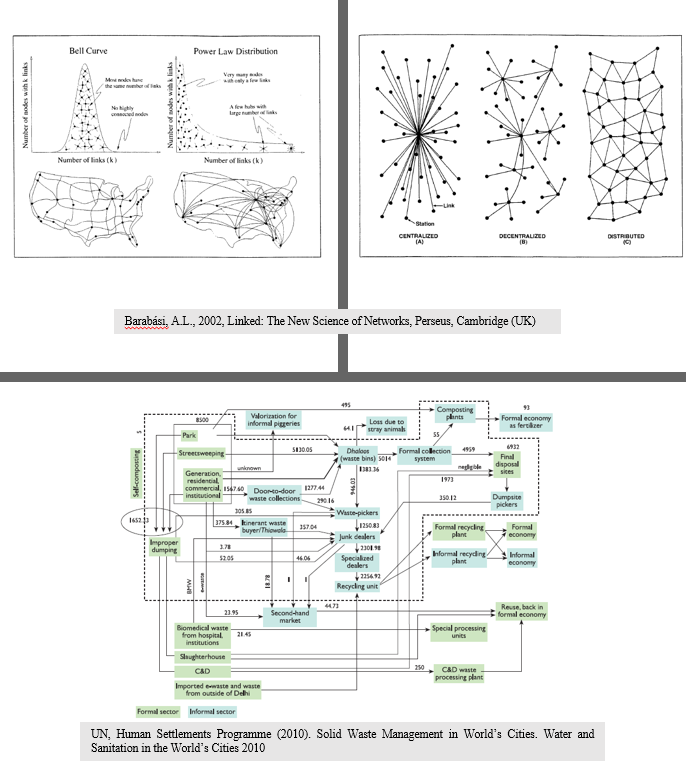
\includegraphics[width=0.5\textwidth]{Imgs/rl_3.PNG}
    \caption{Research Lines 3}
    \label{fig:rl3}
\end{figure}





\subsection{The Role of Location to enhance Circular Economy in the City-Region}
\textbf{\underline {Short Project Description:}} After revealing industry’s needs, products and waste materials, it’s important to understand their location. By mapping and modelling the spatial relationship of different industries or businesses opportunities for potential synergies can be detected. Moreover, previously unseen demands could be seen by looking at how activities are distributed in space.  \par


\textbf{\underline {Hypothesis:}}  Circular Economy performance is space dependent and by modelling socio-economic activities is space, circularity can be enhanced.  \par


\textbf{\underline {Exploratory Research Questions: }}  
\begin{itemize}
    \item Model the system to identify potential opportunities and threats.
    \item How to integrate these into the planning process to improve these systems?
    \item Is the functioning of these systems affected by spatial planning?
\end{itemize}

\begin{figure}[hbt!]
    \centering
    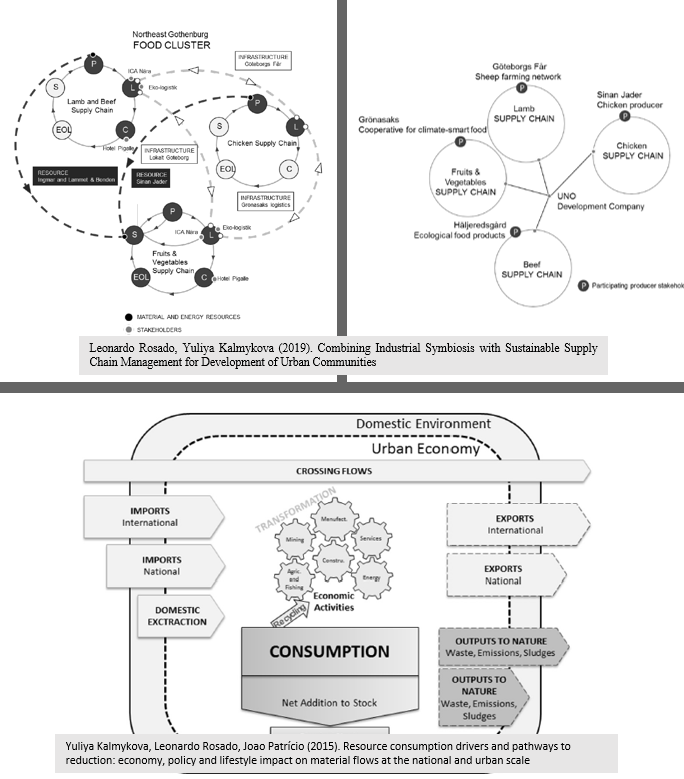
\includegraphics[width=0.5\textwidth]{Imgs/rl_4.PNG}
    \caption{Research Lines 4}
    \label{fig:rl4}
\end{figure}




\subsection{Integration between the food System and waste MGMT}
\textbf{\underline {Short Project Description:}} To some extent, waste MGMT and food system could be integrated into one system. Food waste could be used as compost or as energy, but the location of farms, warehouses and recycling facilities might contribute or undermine the synergies between these systems. \par

The mapping and analysis of these systems is not a straightforward task. There are multiple actors and they might be represented at different geographical and temporal scales. Aggregating and modelling these systems for a product will allow to understand how different actions or events can affect the overall performance of the system.  \par

This project will track different components or subcomponents to reveal the spatial cycle as the move around the metabolic cycle of city-regions. \par



\textbf{\underline {Hypothesis:}} Aggregating the relationships between different actors across different spatial-temporal scales will enable to plan better city-regions. The spatial patterns hold valuable information for Planning processes. By revealing the flow of components, materials or inputs, it would be able to identify potential opportunities or threats of the system. \par


\textbf{\underline {Exploratory Research Questions: }} 
\begin{itemize}
    \item How to (dis)aggregate and connect the different operators’ levels?
    \item What is the effect of changes in the system?
    \item How does actions propagate across levels?
\end{itemize}

\begin{figure}[hbt!]
    \centering
    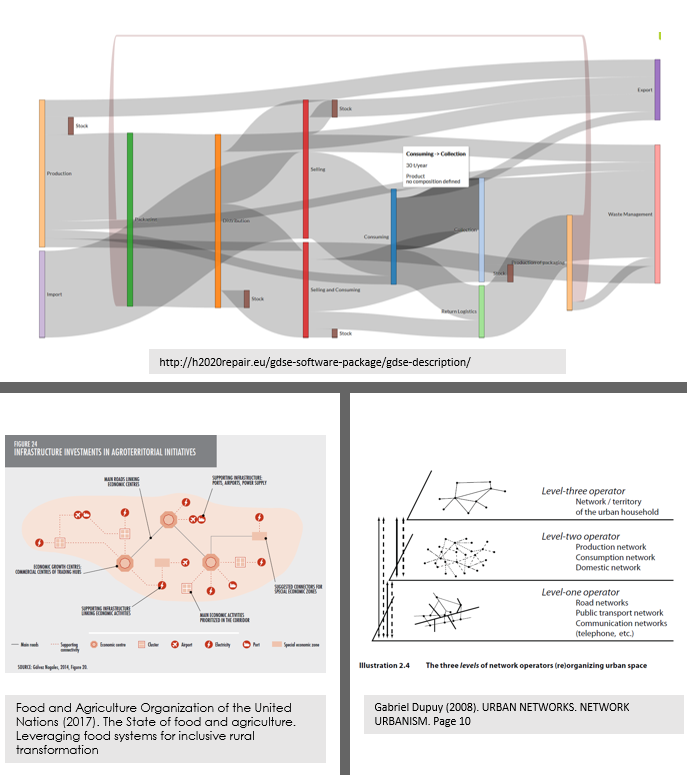
\includegraphics[width=0.5\textwidth]{Imgs/rl_5.PNG}
    \caption{Research Lines 5}
    \label{fig:rl5}
\end{figure}


